%%%%%%%%%%%%%%%%%%%%%%%%%%%%%%%%%%%%%%%%%%%%%%%%%%%%%%%%%%%%%%%%%%%%
%% I, the copyright holder of this work, release this work into the
%% public domain. This applies worldwide. In some countries this may
%% not be legally possible; if so: I grant anyone the right to use
%% this work for any purpose, without any conditions, unless such
%% conditions are required by law.
%%%%%%%%%%%%%%%%%%%%%%%%%%%%%%%%%%%%%%%%%%%%%%%%%%%%%%%%%%%%%%%%%%%%

\documentclass{beamer}
\usetheme[faculty=phil]{fibeamer}
\usepackage[utf8]{inputenc}
\usepackage[
  main=english
]{babel}
%% These macros specify information about the presentation
\title{Classical Black Holes} %% that will be typeset on the
\subtitle{11. Novikov-Thorne Thin Disks  } %% title page.
\author{Edward Larra\~{n}aga}
%% These additional packages are used within the document:
\usepackage{ragged2e}  % `\justifying` text
\usepackage{booktabs}  % Tables
\usepackage{tabularx}
\usepackage{tikz}      % Diagrams
\usetikzlibrary{calc, shapes, backgrounds}
\usepackage{amsmath, amssymb}
\usepackage{url}       % `\url`s
\usepackage{listings}  % Code listings
\usepackage{siunitx}
\frenchspacing
\begin{document}
\frame{\maketitle}

\AtBeginSection[]{% Print an outline at the beginning of sections
\begin{frame}<beamer>
\frametitle{Outline for Part \thesection}
\tableofcontents[currentsection]
\end{frame}}


\section{Novikov-Thorne Thin Disk}    

\begin{frame}
\Huge
Novikov-Thorne Thin Disks
\end{frame}

\begin{frame}{Novikov-Thorne Thin Disks}
	\begin{itemize}
	\item Geometrically thin and optically thick accretion disk.
	\pause
	\item Has four parameters: BH mass, BH spin, mass accretion rate and viscosity parameter.
	\end{itemize}		
\end{frame}

\begin{frame}{Novikov-Thorne Thin Disks}
	\begin{itemize}
	\item The spacetime is stationary, axisymmetric, asymptotically flat, and reflection- symmetric with respect to the equatorial plane.
	\pause
	\item The accretion disk is non-self-gravitating; that is, the impact of the disk’s mass on the background metric is ignored.
	\pause
	\item The accretion disk is in the equatorial plane; that is, the disk is perpendicular to the black hole spin.
	\pause
	\item The inner edge of the disk is at the ISCO radius.
	\end{itemize}		
\end{frame}

\begin{frame}{Modeling Viscosity}
	\begin{center}
      \begin{figure}
      	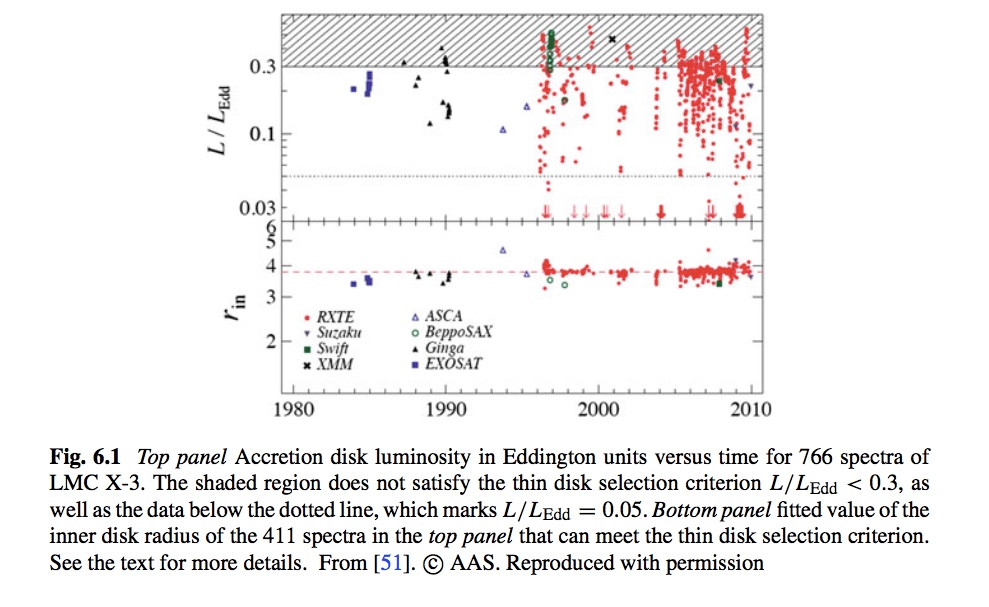
\includegraphics[scale=0.3] {figures/LMCX3ISCO.jpeg}
      \end{figure}
	\end{center}	
\end{frame}


\begin{frame}{Novikov-Thorne Thin Disks}
	\begin{itemize}
	\item The accretion disk is geometrically thin, namely the disk opening angle is $h/r\ll
1$ , where $h(r)$ is the semi-thickness of the disk at the radial coordinate $r$ .
	\pause
	\item We suppose to average over time scales $\Delta t$ that are short enough to assume that the spacetime is stationary (for instance, the mass accreted by the central object does not appreciable change the background metric) and large enough to neglect possible inhomogeneities in the accretion fluid.\\
	\pause
	Any physical quantity $\Psi (t, r, \theta, phi)$ will be averaged over $t$ and $\phi$,
	\[\Psi (r,\theta) = \frac{1}{2 \pi \Delta t} \int_0 ^{\Delta t} \int _0 ^{2\pi} \Psi (t, r, \theta, \phi) d\phi dt \]
	\end{itemize}		
\end{frame}

\begin{frame}{Novikov-Thorne Thin Disks}
	\begin{itemize}
	\item The particles of the gas follow nearly-geodesic circular orbits in the equatorial
plane.
	\pause
	\item Radial heat transport is ignored, and energy and angular momentum are radiated from the disk surface.\\
	\pause
	This assumption requires a thin accretion disk.
	\pause
	\item Magnetic fields are ignored.
	\end{itemize}		
\end{frame}

\begin{frame}{Novikov-Thorne Thin Disks}
	\begin{itemize}
	\item Energy and angular momentum from the disk's surface are only carried away by photons with wavelength $\lambda \ll M$.\\
	\pause
	This assumption let us neglect possible coherent superpositions of  radiation reaction in nearby regions of the disk.
	\pause
	\item The effect of energy and angular momentum transport by photons emitted from the disk and returning to the disk due to strong light bending in the vicinity of the black hole (returning radiation) is neglected.
	\end{itemize}		
\end{frame}

\subsection{Thin Disk General Description}
\begin{frame}
\Huge
Thin Disk General Description
\end{frame}

\begin{frame}{Thin Disk General Description}
	\begin{itemize}
	\item The time-averaged radial structure of the Novikov-Thorn disk is obtained from the conservation laws (energy, angular momentum and rest mass)
	\pause
	\item The description will be independent of the specific properties of the accretion.
	\end{itemize}
\end{frame}

\begin{frame}{Mass Accretion Rate}
	Conservation of the rest mass:
	\pause
	\[\nabla _\mu (\rho u^\mu) = 0 \]
	\pause
	$\rho$: Time-averaged rest mass density\\
	$u^\mu$: Time-averaged 4-velocity of the fluid
\end{frame}

\begin{frame}{Thin Disk General Description}
	Integrating over the 3-volume of the disk (between $r$ and $r + \Delta r$) and using Gauss' theorem,
	\pause	
	\[ \dot{M} = -2\pi \sqrt{-\gamma} \Sigma u^r = \textrm{constant} \]
	\pause
	$\gamma = - \left( \frac{g^2_{t\phi}}{g_{\phi \phi}} - g_{tt} \right) g_{rr} g_{\phi \phi}$\\
	\bigskip
	
	$\Sigma (r) = \int _{-h} ^h \rho dz$
\end{frame}

\begin{frame}{Energy Flux and Torque}
	From the conservation of energy,
	\[\nabla _\mu T^{t\mu} = 0\]
	and angular momentum,
	\[\nabla _\mu T^{\phi \mu} = 0\]
\end{frame}

\begin{frame}{Energy Flux and Torque}
	we obtain the time-averaged energy flux emitted from the surface of the disk,
	\[ \mathcal{F} (r) = \frac{\dot{M}}{4\pi M^2} F(r)\]
	\pause
	and the time-averaged torque,
	\[ W^r _\phi (r) = \frac{\dot{M}}{2\pi M^2} \frac{(\Omega \ell_z - \varepsilon)}{\partial_r \Omega} F(r)\]
	\pause
	$\varepsilon$: specific energy\\
	$\ell_z$: specific axial component of the angular momentum\\
	$\Omega$: Angular velocity for equatorial circular geodesics
\end{frame}


\begin{frame}{Energy Flux and Torque}
	\[ F(r) = - \frac{\partial_r \Omega}{(\varepsilon - \Omega \ell_z )^2} \frac{M^2}{\sqrt{-\gamma}} 
	\int_{r_{in}} ^r \left[ (\varepsilon - \Omega \ell_z ) \partial_x \ell_z \right] dx \]
	\pause
	$r_{in}$: inner edge of the disk (presumably the ISCO radius)
\end{frame}

\begin{frame}{Efficiency}
	\[L_{acc} = \eta \dot{M}\]
	\pause
	$\eta$: Total efficiency
	\pause
	\[ \eta = \eta_r + \eta_k\]
	\pause
	$\eta_r$: Radiative Efficiency (can be measured form bolometric luminosity)
	\pause
	\[ L_{bol} = \eta_r \dot{M}\]
\end{frame}

\begin{frame}{Efficiency}
	\[L_{acc} = \eta \dot{M}\]
	$\eta$: Total efficiency
	\[ \eta = \eta_r + \eta_k\]
	\pause
	$\eta_k$: gravitational energy transformed into kinetic energy of jets or outflows\\
	\pause
	For Novikov-Thorn disks: $\eta_k = 0$\\
	\pause
	\[\eta_{NT} = \eta_r\]
\end{frame}


\begin{frame}{Efficiency}
	\begin{itemize}
	\item The particles of the accreting gas slowly fall onto the BH
	\pause
	\item When particles reach the ISCO radius, they quickly plunge onto the BH without emitting additional radiation
	\pause
	\item A fraction of the emitted radiation is captured by the BH
	\end{itemize}
	\pause
	\[\eta_NT = 1 - \varepsilon_{ISCO} - \zeta \]
	\pause
	$\varepsilon_{ISCO}$: Specific energy of a test particle at the ISCO\\
	$\zeta$: Fraction of energy captured by the BH
\end{frame}

\begin{frame}{Efficiency}
	\[ \zeta = \frac{1}{\dot{M}} \int _{r_{ISCO}} ^\infty \left[ \int_0^{\pi /2} \int_0^{2\pi} C \Upsilon (-n_t) \cos \theta \sin \theta d\phi d\theta \right] \mathcal{F} (r) 4r dr \]
	\pause
	\[ C =	
	\begin{cases}
		0 &\textrm{ radiation escapes}\\
		1 &\textrm{ radiation is captured}\\
	\end{cases}\]
\end{frame}

\begin{frame}{Efficiency}
	\[ \zeta = \frac{1}{\dot{M}} \int _{r_{ISCO}} ^\infty \left[ \int_0^{\pi /2} \int_0^{2\pi} C \Upsilon (-n_t) \cos \theta \sin \theta d\phi d\theta \right] \mathcal{F} (r) 4r dr \]
	\pause
	$\Upsilon$: takes into account possible angular dependence of the emission
	\[ 	
	\begin{cases}
		\Upsilon = 1 &\textrm{ isotropic emission}\\
		\Upsilon \propto 1+2\cos \theta &\textrm{ limb-darkened emission}\\
		... & 
	\end{cases}\]
\end{frame}

\begin{frame}{Efficiency}
	\[ \zeta = \frac{1}{\dot{M}} \int _{r_{ISCO}} ^\infty \left[ \int_0^{\pi /2} \int_0^{2\pi} C \Upsilon (-n_t) \cos \theta \sin \theta d\phi d\theta \right] \mathcal{F} (r) 4r dr \]
	\pause
	$n^\mu$: normalized photon 4-momentum
	\[ n^\mu = \frac{k^\mu }{k_{(t)}}\]
	$k^\mu$: photon 4-momentum\\
	$k_{(t)}$: photon energy in the rest frame of the emitter
\end{frame}


\subsection{Kerr Spacetime}    

\begin{frame}
\Huge
Kerr Spacetime
\end{frame}

\begin{frame}{Kerr Spacetime}
	\[ \varepsilon = \frac{r^{3/2} - 2Mr^{1/2} \pm aM^{1/2}}{r^{3/4} \sqrt{r^{3/2} - 3Mr^{1/2} \pm 2aM^{1/2}}} \]
	\pause
	\[ \ell_z = \pm \frac{M^{1/2} \left( r^2 \mp 2aM^{1/2}r^{1/2} + a^2\right) }{r^{3/4} \sqrt{r^{3/2} - 3Mr^{1/2} \pm 2aM^{1/2}}} \]
	\pause
	\[ \Omega_{\pm} = \pm \frac{M^{1/2}}{r^{3/2} \pm aM^{1/2}} \]
	\pause
	\[ \sqrt{-\gamma} = r \]
\end{frame}

\begin{frame}{Kerr Spacetime}
	\begin{align*}
	F(x) = & \frac{3}{2} \frac{1}{x^4 ( x^3 -3x + 2a)} \left[x - x_0 -\frac{3}{2} a \ln \left( \frac{x}{x_0} \right) \right. \\
	& -\frac{3(x_1 - a)^2}{x_1 (x_1 - x_2)(x_1-x_3)} \ln \left( \frac{x-x_1}{x_0-x_1} \right)\\
	& - \frac{3(x_2 - a)^2}{x_2 (x_2 - x_1)(x_2-x_3)} \ln \left( \frac{x-x_2}{x_0-x_2} \right)\\
	& \left. - \frac{3(x_3 - a)^2}{x_3 (x_3 - x_1)(x_3-x_2)} \ln \left( \frac{x-x_3}{x_0-x_3} \right)\right]
	\end{align*}	 
\end{frame}

\begin{frame}{Radial Structure Evolution}
	$x= \sqrt{\frac{r}{M}}$\\
	$x_0= \sqrt{\frac{r_{ISCO}}{M}}$\\
	$x_1$, $x_2$ and $x_3$ are the roots of $x^3 - 3x + 2a=0$,\\
	\pause
	\bigskip
	
	$x_1 = 2\cos\left( \frac{1}{3} \arccos a - \frac{\pi}{3} \right)$\\
	$x_2 = 2\cos\left( \frac{1}{3} \arccos a + \frac{\pi}{3} \right)$\\
	$x_3 = -2\cos\left( \frac{1}{3} \arccos a  \right)$

\end{frame}

\begin{frame}{Radiative Efficiency in Kerr spactime}
	Neglecting the radiation captured by the BH, $\zeta = 0$ the NT efficiency is $\eta_{NT} = 1 - \varepsilon_{ISCO} $\\
	
	\pause
	where $\varepsilon_{ISCO}$ is 
	\[ \varepsilon = \frac{r^{3/2} - 2Mr^{1/2} \pm aM^{1/2}}{r^{3/4} \sqrt{r^{3/2} - 3Mr^{1/2} \pm 2aM^{1/2}}} \]
	\pause
	evaluated at\\
	$r_{ISCO} = 3M + Z_2 \mp \sqrt{(3M-Z_1)(3M+Z_1+2Z_2)} $\\
	\bigskip
	\pause
	$Z_1 = M + (M^2-a^2)^{1/3} [(M+a)^{1/3} + (M-a)^{1/3} ]$\\
	\pause
	$Z_2 = \sqrt{3a^2 +Z_1^2} $ 
\end{frame}

\begin{frame}{Radiative Efficiency in Kerr spactime}
	\[\eta_{NT} = \eta_{NT} (a) \]
	\pause
	Particular cases:
	\pause
	\[\eta_{NT} (a=0) = 0.057 \]
	\pause
	\[\eta_{NT} (a=1) = 0.423 \textrm{ (co-rotating disk)} \]
	\pause
	\[\eta_{NT} (a=1) = 0.038 \textrm{ (counter-rotating disk)} \]
\end{frame}

\begin{frame}{Formation of the Accretion Disk}
	\begin{center}
      \begin{figure}
      	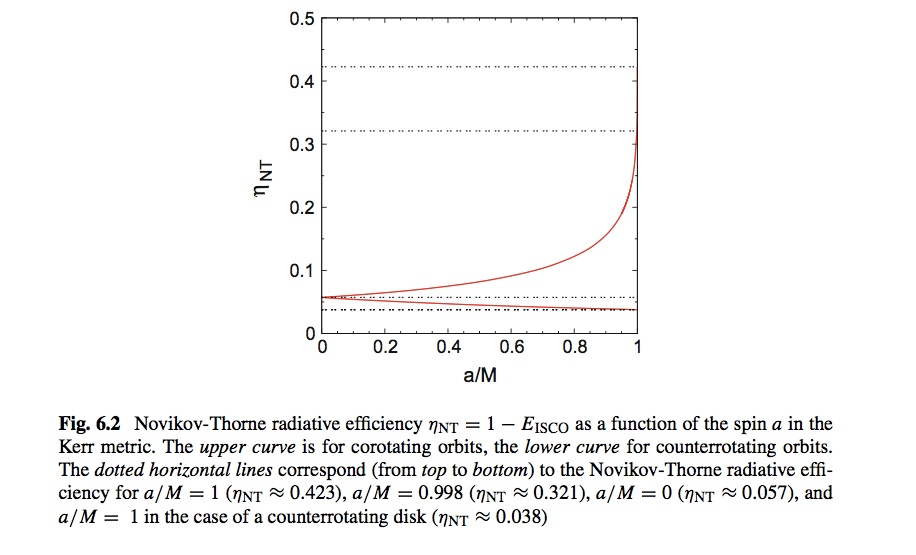
\includegraphics[scale=0.35] {figures/Efficiency.jpeg}
      \end{figure}
	\end{center}	
\end{frame}


\section{Transfer Function and Spectrum for Thin Disks}    
\begin{darkframes}

\begin{frame}
\Huge
Transfer Function
\end{frame}

\begin{frame}{Spectrum of the Thin Accretion Disk}
	The spectrum produced by a thin accretion disk is calculated by using the \textit{transfer function} and considering two parts in the calculation,
	\pause
	\begin{itemize}
	\item The first part corresponds to find the local spectrum (radiation at the surface of the accretion disk)
	\pause
	\item The second part corresponds to describe the propagation of the radiation from the disk to observer
	\end{itemize}		
\end{frame}

\begin{frame}{Local Spectrum}
	\begin{itemize}
	\item The local spectrum of the radiation depends only on the astrophysical model (it does not depend on the spacetime geometry)
	\pause
	\item The local spectrum will be given by the specific intensity $I_e (\nu_e, r_e, \vartheta_e)$\\
	\pause
	\bigskip
	
	$\nu_e$: emitted photon frequency (in the rest frame of the disk)\\
	$r_e$: emission radius\\
	$\vartheta_e$: emission angle with respect to the normal to the disk
	\end{itemize}		
\end{frame}

\end{darkframes}

\begin{frame}{Formation of the Accretion Disk}
	\begin{center}
      \begin{figure}
      	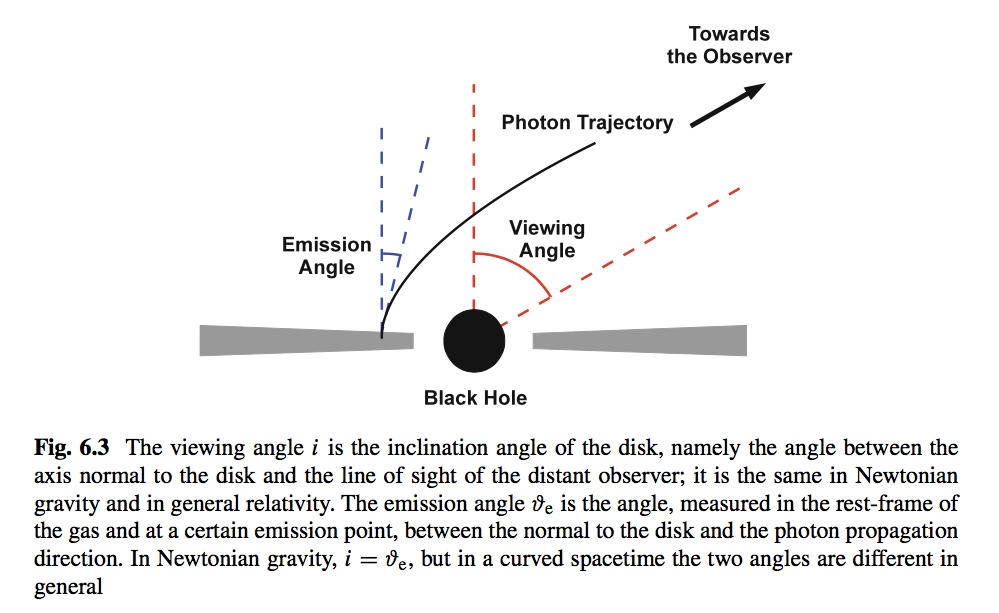
\includegraphics[scale=0.3] {figures/emissionAngle.jpeg}
      \end{figure}
	\end{center}	
\end{frame}

\begin{darkframes}

\begin{frame}{Observed Spectrum}
	The observed flux (in units of $\textsf{ erg s}^{-1} \textsf{ cm}^{-2} \textsf{ Hz}^{-1}$ )
	\[ F_{obs} (\nu_{obs}) = \int I_{obs} (\nu_{obs}, X,Y) d \tilde{\Omega} \]	
	\pause
	$I_{obs}$: Specific intensity detected by the observer\\
	$d\tilde{\Omega} = \frac{dXdY}{D^2}$: Element of solid angle subtended by the image of the disk in the observer's sky\\
	$D$: Distance observer-source\\
	\pause 
	\[ F_{obs} (\nu_{obs}) = \int g^3 I_e (\nu_e, r_e, \vartheta_e) d \tilde{\Omega} \]
	\pause
	$ g = \frac{\nu_{obs}}{\nu_e} $: redshift factor
	\pause
	\[ I_{obs} = g^3 I_e \]
\end{frame}

\begin{frame}{The transfer function}
	\begin{itemize}
	\item In order to describe the spacetime geometry information and the position of the observer, we introduce the \textit{transfer function}, $ f(g^*, r_e, i) $. 
	\pause
	\item This function includes all the relativistic effects such as gravitational and Doppler redshift, light bending, etc.
	\pause
	\[ g^* = \frac{g-g_{min}}{g_{max} - g_{min}}\]
	\pause
	$ g_{max} = g_{max} (r_e, i )$: maximum value of the redshift factor\\
	$ g_{min} = g_{min} (r_e, i )$: minimum value of the redshift factor
	\end{itemize}		
\end{frame}

\begin{frame}{The transfer function}
	\[ F_{obs} (\nu_{obs}) = \int g^3 I_e (\nu_e, r_e, \vartheta_e) d \tilde{\Omega} \]
	\pause
	\[ F_{obs} (\nu_{obs}) = \frac{1}{D^2} \int \int g^3 I_e (\nu_e, r_e, \vartheta_e) dXdY \]
	\pause
	\[ F_{obs} (\nu_{obs}) = \frac{1}{D^2} \int_{r_{ISCO}} ^\infty \int_0 ^1  \frac{\pi r_e g^2}{\sqrt{g^* (1-g^*)}} f(g^*, r_e , i) I_e (\nu_e, r_e, \vartheta_e) dg^* dr_e \]
	\pause
	\[f(g^*, r_e, i ) = \frac{1}{\pi r_e} g \sqrt{g^* (1-g^*)} \left| \frac{\partial (X,Y)}{\partial (g^*, r_e)}\right| \]
\end{frame}

\begin{frame}{Explicit form of the transfer function}
	\begin{itemize}
	\item Consider a stationary and axisymmetric spacetime. 
	\pause
	\item We need to relate the position of the received photon, $(X,Y)$ with the emission point, $r_e$, and with the redshift factor ,$g$, and the emission angle, $\vartheta$.
	\pause
	\item This relation is obtained by evolving (numerically) the geodesic equations from the observation point to the emission point.
	\end{itemize}
\end{frame}

\begin{frame}{Explicit form of the transfer function. Redshift}
	\begin{itemize}
	\item Numerically solving the geodesic equations give the position of the emitted photon in the accretion disk, $r_e$ 
	\pause
	\item The redshif factor is defined as the relation between the measured frequency (in the observer's frame) and the emitted frequency (in the rest frame of the gas)
	\pause
	\[ g = \frac{\nu_{obs}}{\nu_e} = \frac{-u^\mu _{obs} k_\mu }{-u^\nu _{e} k_\nu }\]
	\pause
	$ u^\mu _{obs} = u^t _e (1,0,0,\Omega)$: 4-velocity of the observer\\
	$ u^\nu _{e} = (1,0,0,0)$: 4-velocity of the gas particles\\ 
	\end{itemize}
\end{frame}

\begin{frame}{Explicit form of the transfer function. Redshift}
	\begin{itemize}
	\item Using the normalization condition $g_{\mu \nu} u_e ^\mu u_e ^\nu = -1$,
	\pause
	\[ g = \frac{\sqrt{-g_{tt} -2 g_{t \phi} \Omega - g_{\phi \phi} \Omega^2 }}{1-\lambda \Omega} \]
	\pause
	$ \lambda = - \frac{k_\phi}{k_t}$\\
	$ k_t = - \varepsilon $: energy of the photon (constant of motion)\\ 
	\end{itemize}
\end{frame}

\begin{frame}{Explicit form of the transfer function. Emission angle}
	\begin{itemize}
	\item Normal to the disk
	\[ n^\mu = \left. \left( 0, 0, \sqrt{g^{\theta \theta}}, 0 \right) \right|_{r_e, \theta_e = \pi / 2}  \]
	\pause
	\item The emission angle is given by
	\[\cos \vartheta_e = \pm \left. \frac{n^\mu k_\mu }{u_e^\nu k_\nu } \right|_e \]
	\pause
	\[\cos \vartheta_e = \pm \sqrt{g^{\theta \theta}}  \frac{\sqrt{-g_{tt} -2 g_{t \phi} \Omega - g_{\phi \phi} \Omega^2 }}{1-\lambda \Omega} \frac{k_\theta}{k_t}\]
	\end{itemize}
\end{frame}

\begin{frame}{Explicit form of the transfer function. Jacobian}
	\begin{itemize}
	\item At the end of the numerical integration of the geodesic equations one has
	\pause
	\begin{align*}
	r_e &= r_e (X,Y)\\
	g &= g(X,Y)\\
	\vartheta &= \vartheta (X,Y)
	\end{align*}
	\pause
	\item From the first two relations we may calculate the Jacobian as
	\[ \left| \frac{\partial (X,Y)}{\partial (g^*, r_e)} \right| = \left( g_{max} - g_{min} \right) \left| \frac{\partial X}{\partial g} \frac{\partial Y}{\partial r_e} - \frac{\partial X}{\partial r_e} \frac{\partial Y}{\partial g} \right|\]
	\end{itemize}
\end{frame}






\end{darkframes}
\begin{frame}{Temperature of the gas in the accretion structure}
	\begin{center}
      \begin{figure}
      	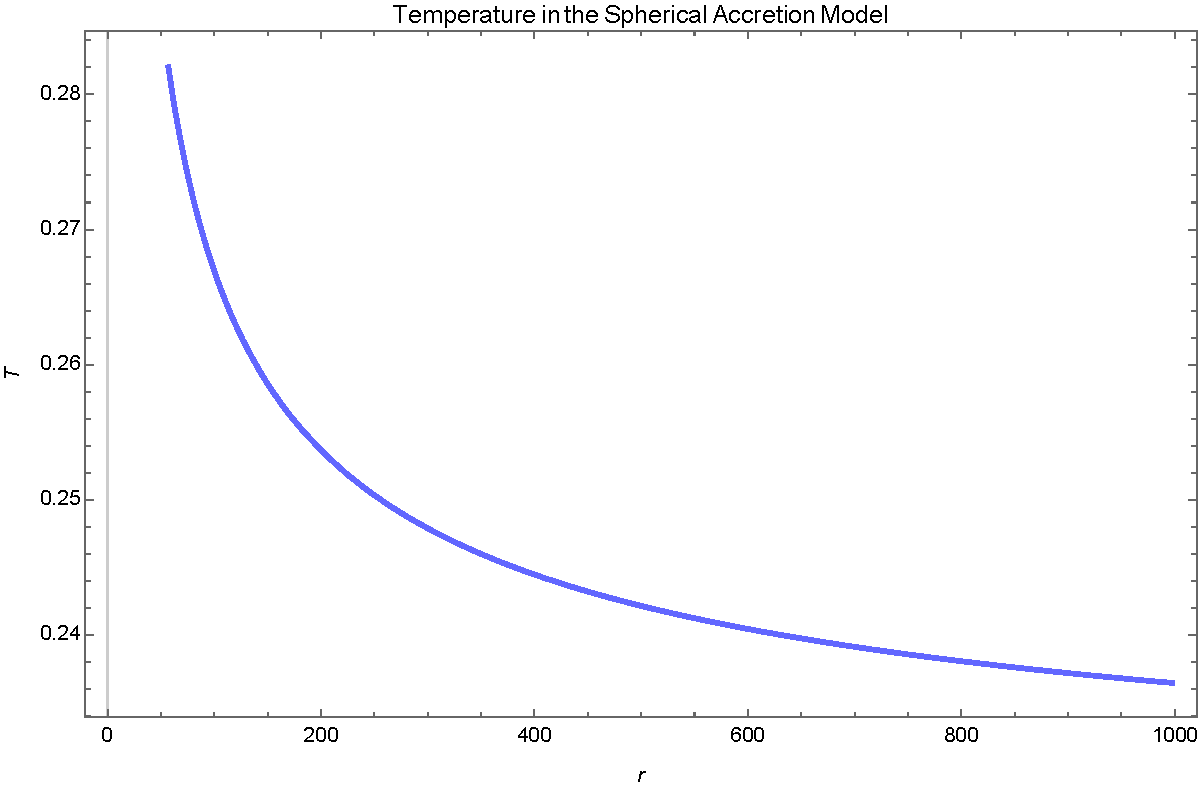
\includegraphics[scale=0.45] {figures/Temperature.pdf}
      \end{figure}
	\end{center}	
\end{frame}

\begin{darkframes}

\begin{frame}{Next Lecture}
  	\Large
	{10. Accretion Disks. Detailed Description}
\end{frame}

  
\end{darkframes}
\end{document}
